\documentclass[hyperref={pdfpagelabels=false}]{beamer}
\usepackage{lmodern}
\usetheme{Frankfurt}
\usecolortheme{crane}
\usepackage[noend]{algorithmic}
\usepackage{tikz}
\usepackage{wrapfig}
\usepackage{lipsum}
\usepackage{sidecap}
\usepackage{graphicx}
\usepackage{subcaption}
\usepackage{float}
\usepackage{amsmath}
\usepackage{hyperref}
\hypersetup{
    colorlinks=true,
    linkcolor=blue,
    filecolor=magenta,      
    urlcolor=cyan,
}
% \usepackage{enumitem}
\usetikzlibrary{shapes,arrows,positioning,calc}
\usetikzlibrary{decorations.pathreplacing}
% below code is used for making diagrams in slides
% do not delete it
\tikzset{
    block/.style = {
        draw, 
        fill=white, 
        rectangle, 
        minimum height=1.8em, 
        minimum width = 10em
    },
    block2/.style = {
        draw, 
        fill=white, 
        rectangle, 
        minimum height=3.7em, 
        minimum width=6em
    },
    sum/.style = {
        draw, 
        fill=white, 
        circle, 
        inner sep=0pt,
        minimum size = 0.5cm
    },
    pinstyle/.style = {
        pin edge={to-,thin,black}
    }
}


\title{PRESENT Cipher}  
\author{\texttt{Thunderspy}} 
\institute{
	
\includegraphics[scale=0.08]{logoiitbh}
	
	Department of \texttt{Electrical Engineering and Computer Science}\\ 
	Indian Institute of Technology Bhilai}

\begin{document}
	\begin{frame}
	\titlepage
    
\end{frame} 

\AtBeginSection[]
{
	\begin{frame}<beamer>
	\frametitle{Outline}
	\tableofcontents[currentsection]
\end{frame}
}

\section{Introduction}


\begin{frame}{The Present Cipher}
\begin{itemize}
    \item Ultra-Lightweight block cipher.
    \item Developed by the Orange Labs (France), Ruhr University Bochum (Germany) and the Technical University of Denmark in 2007.
    \item Supports 64 bits block size and 80 or 128 bits key sizes with 31 rounds.
    \item Intended to be used in circumstances where high chip performance and low power consumption are required. 
\end{itemize}
\end{frame}

\begin{frame}{Substitution/ Permutation}
\begin{figure}[H]
    \centering
    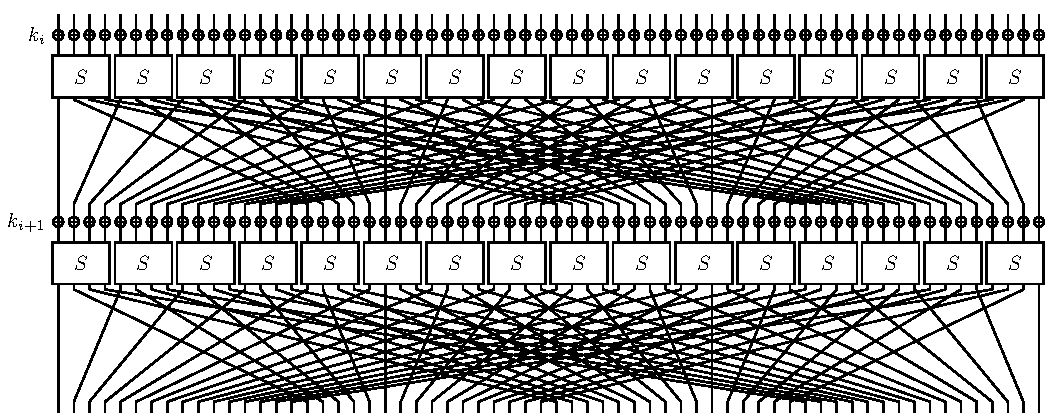
\includegraphics[width=\linewidth]{PRESENT_diagram.pdf}
\end{figure}
\begin{center}
    \scalebox{0.95}{
    \begin{tabular}{ |c||c|c|c|c|c|c|c|c|c|c|c|c|c|c|c|c| }
        \hline
        $x$ & 0 & 1 & 2 & 3&4& 5& 6&7&8&9&A&B&C&D&E&F  \\ \hline
        $S[x]$& C & 5 & 6& B &9 &0 &A &D& 3& E &F& 8& 4 &7& 1& 2 \\ \hline
    \end{tabular}}\\
    Image source : iacr.org/authors/tikz/
\end{center}
\end{frame}
\section{Cipher Specifications}

\begin{frame}[c]{Cipher Design}
\begin{itemize}
    \item PRESENT-80 is an example of SP-network.
    \item 4-bit S-Box is applied 16 times in parallel for the 64-bit input during each round.
    \begin{block}{High level psuedo-code of PRESENT algorithm}
        \begin{algorithmic}[1]
        \STATE{generateRoundKeys()}
        \FOR{$i=1$ \TO $31$ }
            \STATE {addRoundKey(\textsc{State},$K_i$)} 
            \STATE {sBoxLayer(\textsc{State})} 
            \STATE {pLayer(\textsc{State})} 
        \ENDFOR
        \STATE addRoundKey(\textsc{State},$K_{32}$)
        \end{algorithmic}
    \end{block}
\end{itemize}
\end{frame}

\begin{frame}{Cipher Design contd.}
    \begin{columns}
    \begin{column}{0.5\textwidth}
       \begin{block}{Add Round Key}
           \begin{itemize}
               \item Round key $K_i = k_{63},k_{62} \dots k_0$ for $1\leq i \leq 32$.
               \item Current state $S = s_{63},s_{62}\dots s_0$.
               \begin{eqnarray*}
                    S \xrightarrow{} S \oplus K_i \\
                    \implies s_t \xrightarrow[]{} s_t \oplus k_t 
                \end{eqnarray*}
                for $0\leq t\leq 63$
           \end{itemize}
       \end{block}
    \end{column}
    \begin{column}{0.5\textwidth}  %%<--- here
        \begin{center}
         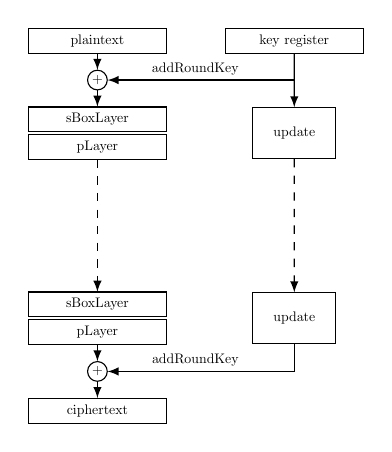
\begin{tikzpicture}[auto, node distance=2cm,>=latex,scale=0.6, every node/.style={scale=0.5}]
            % nodes
            \node [sum] (sum1) {+};
            \node [block,above of=sum1,node distance=1cm] (plaintext) {plaintext};
            \node [block,right of=plaintext,node distance=5cm] (keyregister) {key register};
            \node [block,below of=sum1,node distance=1cm] (sBoxLayer) {sBoxLayer};
            \node [block,below of=sBoxLayer,node distance=0.7cm] (pLayer) {pLayer};
            \node [block,below of=pLayer,node distance=4cm] (sBoxLayer2) {sBoxLayer};
            \node [block,below of=sBoxLayer2,node distance=0.7cm] (pLayer2) {pLayer};
            \node [sum, below of=pLayer2,node distance=1cm] (sum2) {+};
            \node [block,below of=sum2,node distance=1cm] (ciphertext) {ciphertext};
            
            \node [block2,below of=keyregister,node distance=2.35cm] (update) {update};
            \node [block2,below of=update,node distance=4.7cm] (update2) {update};
        
            % arrows
            \draw [->] (plaintext) -- (sum1);
            \draw [->] (sum1) -- (sBoxLayer);
            \draw [->] (pLayer2) -- (sum2);
            \draw [->] (sum2) -- (ciphertext);
            \draw [->] (keyregister) -- (update);
            \draw [->,dashed] (update) -- (update2);
            \draw [->,dashed] (pLayer) -- (sBoxLayer2);
            \draw [->] (keyregister)  |- node[above left= 0pt] {addRoundKey            }    (sum1);
            \draw [->] (update2) |- node[above left= 0pt]{addRoundKey            }   (sum2);
        \end{tikzpicture}
         \end{center}
    \end{column}
    \end{columns}
\end{frame}

\begin{frame}{Substitution Layer $S:\mathbb{F}_2^4\xrightarrow[]{}\mathbb{F}_2^4$}
    Denote Fourier coefficient of S-Box. 
    \begin{equation}
        S_b^W (a) = \sum_{x \in \mathbb{F}_2^4} (-1)^{\langle b,S(x)\rangle + \langle a,x\rangle}
    \end{equation}
     PRESENT S-Box satisfies the following conditions.
    \begin{itemize}
        \item For any fixed input difference $\Delta_I \in \mathbb{F}_2^4,\Delta_I \not = 0$ and output difference $\Delta_O \in \mathbb{F}_2^4,\Delta_I \not = 0$, the following condition is satisfied
        \begin{equation*}
            |\{ x \in \mathbb{F}_2^4~~ \vert~~ S(\Delta_I +x) + S(x) = \Delta_O \}| \leq 4
        \end{equation*}
        \item For any fixed input difference $\Delta_I \in \mathbb{F}_2^4,\Delta_I \not = 0$ and output difference $\Delta_O \in \mathbb{F}_2^4$ such that $wt(\Delta_O) = wt(\Delta_I) = 1$, the following condition is satisfied
        \begin{equation*}
            \{ x \in \mathbb{F}_2^4~~ \vert~~  S(\Delta_I +x) + S(x) = \Delta_O  \} = \Phi
        \end{equation*}
        where $wt(x)$ is the hamming weight of $x$.
    \end{itemize}
\end{frame}
\begin{frame}{Cipher Design Contd.}
    \begin{itemize}
        \item For all $a \in \mathbb{F}_2^4, a \not = 0 $ and $b \in \mathbb{F}_4$, $|S_b^W (a)| \leq 8$ holds.
        \item For all $a \in \mathbb{F}_2^4, a \not = 0 $ and $b \in \mathbb{F}_4$ such that $wt(b) = wt(a) = 1$, $S_b^W (a) = \pm 4 $ holds.
    \end{itemize}
    \begin{block}{Permutation Layer}
        \begin{itemize}
            \item Bit permutation.
            \item Bit $i$ of \textsc{STATE} is moved to bit position $P(i)$.
        \end{itemize}
        \begin{eqnarray*}
         P(i) =  \begin{cases} 
              16.i~~ mod~~ 63 & i \in \{0,1,\dots 62 \}\\
              63 & i = 63 
           \end{cases}
        \end{eqnarray*}
    \end{block}
\end{frame}
\begin{frame}{Key schedule Algorithm}
     We discuss the 80-bit key schedule algorithm.
     \\
     \hspace{40pt}
    \scalebox{0.65}{
    \begin{figure}

        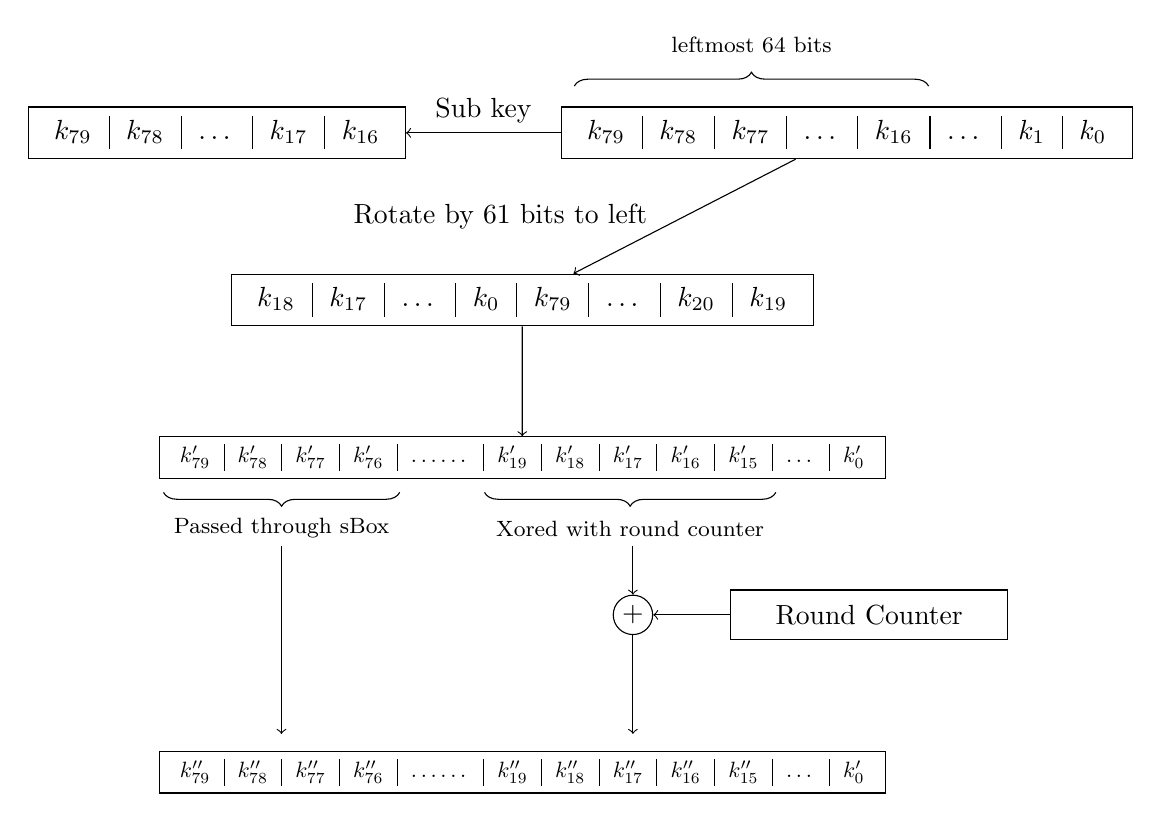
\begin{tikzpicture}
            % nodes
            
            \node (masterkey) [shape = rectangle,draw] {
                \begin{tabular}{c|c|c|c|c|c|c|c}
                    $k_{79}$&$k_{78}$&$k_{77}$&\dots&$k_{16}$&\dots&$k_1$&$k_0$
                \end{tabular}
            };
            \node (subkey) [left of = masterkey,node distance=8cm, shape = rectangle,draw] {
                \begin{tabular}{c|c|c|c|c}
                    $k_{79}$&$k_{78}$&\dots&$k_{17}$&$k_{16}$
                \end{tabular}
            };
            \node (shiftedkey) [below left of =  masterkey,node distance=1cm,shape = rectangle,draw,node distance = 3cm,xshift = -2cm] {
                \begin{tabular}{c|c|c|c|c|c|c|c}
                    $k_{18}$&$k_{17}$&\dots&$k_{0}$&$k_{79}$&\dots&$k_{20}$&$k_{19}$
                \end{tabular}
            };
            \node (shiftedkey2) [below of =  shiftedkey,shape = rectangle,draw,node distance = 2cm,scale = 0.8] {
                \begin{tabular}{c|c|c|c|c|c|c|c|c|c|c|c}
                    $k_{79}'$&$k_{78}'$&$k_{77}'$&$k_{76}'$&\dots\dots&$k_{19}'$&$k_{18}'$&$k_{17}'$&$k_{16}'$&$k_{15}'$&\dots&$k_{0}'$
                \end{tabular}
            };
            
            \node(xor) [sum,below of = shiftedkey2,xshift = 40pt,node distance = 2cm ] {+};
            \node [block,right of=xor,node distance=3cm] (roundCounter) {Round Counter};
            \node (final) [below of =  shiftedkey2,node distance=4cm,shape = rectangle,draw,scale = 0.8] {
                \begin{tabular}{c|c|c|c|c|c|c|c|c|c|c|c}
                    $k_{79}''$&$k_{78}''$&$k_{77}''$&$k_{76}''$&\dots\dots&$k_{19}''$&$k_{18}''$&$k_{17}''$&$k_{16}''$&$k_{15}''$&\dots&$k_{0}'$
                \end{tabular}
            };
            \node (temp1) [below of= shiftedkey2,xshift = -87] {};
            \node (temp2) [below of= shiftedkey2,xshift = -87,yshift = -75] {};
            \node (temp3) [below of= shiftedkey2,xshift = 40] {};
            \node (temp4) [below of= shiftedkey2,xshift = 40,yshift = -75] {};
            
             % arrows
             \draw [decorate,decoration={brace,amplitude=5pt},xshift=-70pt,yshift=-40pt,rotate=180]
             (1,-2) -- (-3.5,-2) node [black,midway,yshift= 15pt] 
             {\footnotesize leftmost 64 bits};
            
             \draw [decorate,decoration={brace,amplitude=5pt},xshift=-190pt,yshift=-73pt]
                (1,-2) -- (-2,-2) node [black,midway,yshift= -13pt] 
                {\footnotesize Passed through sBox};
                
            \draw [decorate,decoration={brace,amplitude=5pt},xshift=-74pt,yshift=-73pt]
            (1.7,-2) -- (-2,-2) node [black,midway,yshift= -13pt] {\footnotesize Xored with round counter};
            
            \draw [->] (masterkey) -- node[above= 0pt]{Sub key}(subkey)  ;
            \draw [->] (masterkey) -- node[left= 10pt]{Rotate by 61 bits to left} (shiftedkey);
            \draw [->] (shiftedkey) -- (shiftedkey2);
            \draw [->] (temp1) -- (temp2);
            \draw [->] (temp3) -- (xor);
            \draw [->] (roundCounter) -- (xor);
            \draw [->] (xor) -- (temp4);
            
             % \draw (nodeXj') -- (nodeD');
        \end{tikzpicture}
    \end{figure}
    }
\end{frame}
\section{DC}

\begin{frame}{Round Reduced Attack}
\begin{figure}[H]
        \centering
        \minipage{\textwidth}
        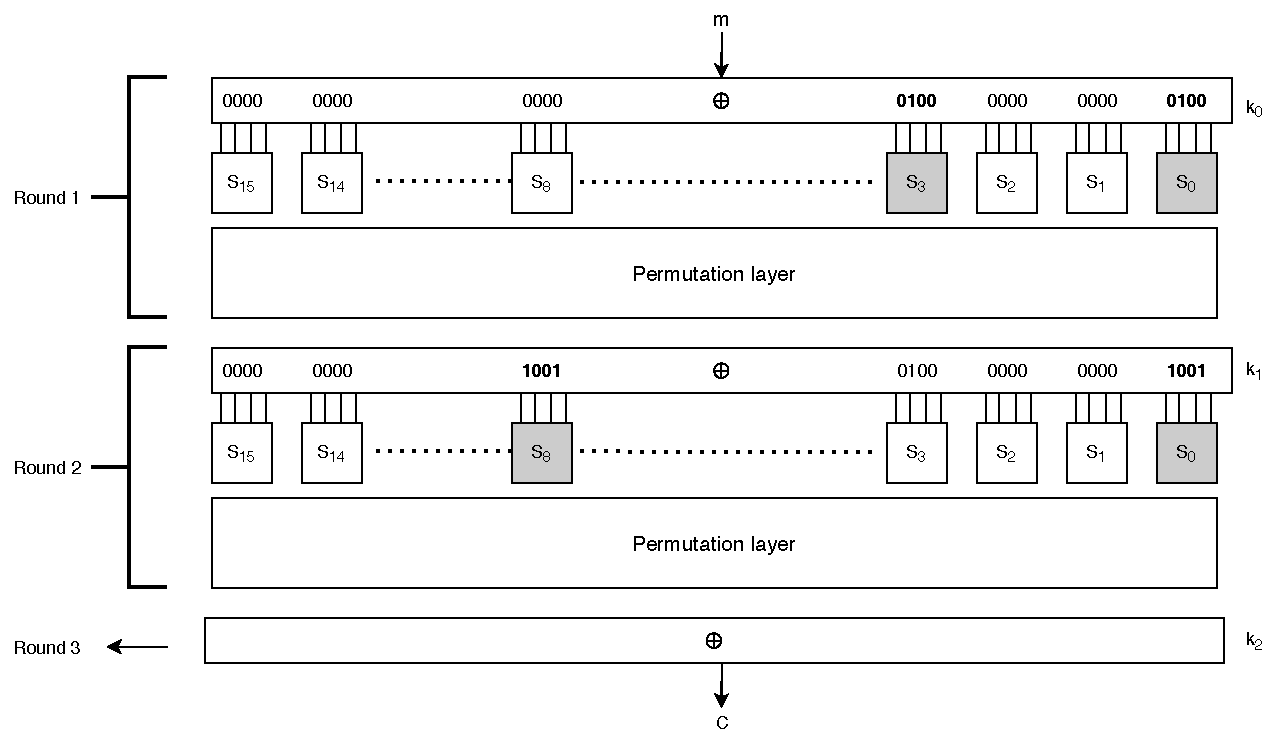
\includegraphics[width=\linewidth]{DC1.pdf}
        \endminipage
        \caption{Attack Model}
    \end{figure}
\end{frame}


\begin{frame}{The Difference Distribution Table}
\begin{figure}[h!]
    \centering
    \scalebox{0.8}{
    \begin{tabular}{ |c||c|c|c|c|c|c|c|c|c|c|c|c|c|c|c|c| }
        \hline
         & 0 & 1 & 2 & 3&4& 5& 6&7&8&9&A&B&C&D&E&F  \\ \hline \hline
         0& 16 & 0 & 0 & 0 &0 &0 &0 &0& 0& 0 &0& 0& 0 &0& 0& 0 \\ 
         1& 0 & 0 & 0 & 4 & 0 & 0 & 0 & 4 & 0 & 4 &0& 0& 0 &4& 0& 0 \\
         2& 0 & 0 & 0 & 2 & 0 & 4 & 2 & 0 & 0 & 0 &2& 0& 2 &2& 2& 0 \\
         3& 0 & 2 & 0 & 2 & 2 & 0 & 4 & 2 & 0 & 0 &2& 2& 0 &0& 0& 0 \\
         4& 0 & 0 & 0 & 0 & 0 & 4 & 2 & 2 & 0 & 2 &2& 0& 2 &0& 2& 0 \\
         5& 0 & 2 & 0 & 0 & 2 & 0 & 0 & 0 & 0 & 2 &2& 2& 4 &2& 0& 0 \\
         6& 0 & 0 & 2 & 0 & 0 & 0 & 2 & 0 & 2 & 0 &0& 4& 2 &0& 0& 4 \\
         7& 0 & 4 & 2 & 0 & 0 & 0 & 2 & 0 & 2 & 0 & 0 & 0 & 2 & 0 & 0 & 4\\
         
         8& 0 & 0 & 0 & 2 & 0 & 0 & 0 & 2 & 0 & 2 & 0 & 4 & 0 & 2 & 0 & 4\\
         9& 0 & 0 & 2 & 0 & 4 & 0 & 2 & 0 & 2 & 0 & 0 & 0 & 2 & 0 & 4 & 0\\
         A& 0 & 0 & 2 & 2 & 0 & 4 & 0 & 0 & 2 & 0 & 2 & 0 & 0 & 2 & 2 & 0\\
         B& 0 & 2 & 0 & 0 & 2 & 0 & 0 & 0 & 4 & 2 & 2 & 2 & 0 & 2 & 0 & 0\\
         C& 0 & 0 & 2 & 0 & 0 & 4 & 0 & 2 & 2 & 2 & 2 & 0 & 0 & 0 & 2 & 0\\
         D& 0 & 2 & 4 & 2 & 2 & 0 & 0 & 2 & 0 & 0 & 2 & 2 & 0 & 0 & 0 & 0\\
         E& 0 & 0 & 2 & 2 & 0 & 0 & 2 & 2 & 2 & 2 & 0 & 0 & 2 & 2 & 0 & 0\\
         F& 0 & 4 & 0 & 0 & 4 & 0 & 0 & 0 & 0 & 0 & 0 & 0 & 0 & 0 & 4 & 4\\ \hline
    \end{tabular}
    }
    \captionof{table}{DDT of the S-box}\label{fig2}
\end{figure}
\end{frame}


\begin{frame}{Differential Characteristics}
\begin{figure}[h!]
        \centering
        \begin{tabular}{ |c||c|c|c| }
            \hline
             Rounds & & Diff. & Prob. \\ \hline \hline
             I& & $x_0 = 4$, $x_4 = 4$ &  \\ 
             $R_1$& $k_0$ & $x_0 = 4$, $x_4 = 4$ & 1 \\
             $R_1$& S & $x_0 = 5$, $x_{3} = 5$ & $2^{-4}$ \\
             $R_1$& P & $x_0 = 9$, $x_{8} = 9$ & 1 \\
             $R_2$& $k_1$ & $x_0 = 9$, $x_{8} = 9$ & 1 \\ \hline
        \end{tabular}
        \captionof{table}{Characteristics}\label{fig7}
    \end{figure}
    \begin{block}{Characteristic}
        ($x_0 = 4$, $x_3 = 4$) $\xrightarrow[]{\text{R}}$ ($x_0 = 9$, $x_8 = 9$)
    \end{block}
\end{frame}

\begin{frame}{Idea of filtering}
    \begin{itemize}
        \item Decrease Wrong pair $\xrightarrow[]{}$ Idea of filtering
        \item Observe from the DDT that transitions from $9 \xrightarrow[]{} \{2,4,6,8,c,e\}$
        \item Thus, after the effect of permutation layer of the second round, $c_1 \oplus c_2$ must belong to the set given below : \\ 
        $\{\{x_4=1,x_6=1\},\{x_6=1,x_8=1\},\{x_4=1,x_6=1,x_8=1\},\{x_6=1,x_{12}=1\},\{x_6=1,x_8=1,x_{12}=1\},...\}$ We have written code for this.
    \end{itemize}
    \begin{block}{Filtering}
        Thus, message pair leading to the cipher text difference other than the above set, can be discarded. 
    \end{block}
\end{frame}

\begin{frame}{Key Guess}
    \begin{figure}[H]
        \centering
        \minipage{\textwidth}
        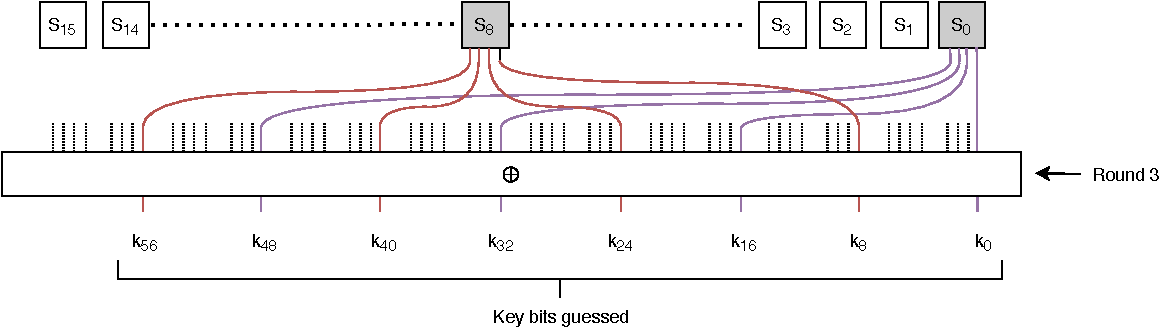
\includegraphics[width=\linewidth]{DC2.pdf}
        \endminipage
        \caption{Attack Model}
    \end{figure}
    \begin{itemize}
        \item Guess 8 bits of the key $k_2$ as shown in the figure.
        \item The probability that the result of partial decryption probabilistically matches $\Delta$out is $<<1$.
        \item Thus, the right guess reaches $\Delta$out more than any other
wrong guess
    \end{itemize}
\end{frame}
\section{LC}

\begin{frame}{The Linear Approximation Table}
\begin{figure}[h!]
    \centering
    \scalebox{0.8}{
    \begin{tabular}{ |c||c|c|c|c|c|c|c|c|c|c|c|c|c|c|c|c| }
        \hline
         & 0 & 1 & 2 & 3&4& 5& 6&7&8&9&A&B&C&D&E&F  \\ \hline \hline
         0& 8 & - & - & - & - & - & - & - & - & - & - & - & - & - & - & - \\ 
         1& - & - & - & - & - & -4 & - & -4 & - & - & - & - & - & -4 & - & 4 \\
         2& - & - & 2 & 2 & -2 & -2 & - & - & 2 & -2 & - & 4 & - & 4 & -2 & 2 \\
         3& - & - & 2 & 2 & 2 & -2 & -4 & - & -2 & 2 & -4 & - & - & - & -2 & -2 \\
         4& - & - & -2 & 2 & -2 & -2 & - & 4 & -2 & -2 & - & -4 & - & - & -2 & 2 \\
         5 & - & - & -2 & 2 & -2 & 2 & - & - & 2 & 2 & -4 & - & 4 & - & 2 & 2\\
         6 & - & - & - & -4 & - & - & -4 & - & - & -4 & - & - & 4 & - & - & -\\
         7 & - & - & - & 4 & 4 & - & - & - & - & -4 & - & - & - & - & 4 & -\\
         8 & - & - & 2 & -2 & - & - & -2 & 2 & -2 & 2 & - & - & -2 & 2 & 4 & 4\\
         9 & - & 4 & -2 & -2 & - & - & 2 & -2 & -2 & -2 & -4 & - & -2 & 2 & - & -\\
         A & - & - & 4 & - & 2 & 2 & 2 & -2 & - & - & - & -4 & 2 & 2 & -2 & 2\\
         B & - & -4 & - & - & -2 & -2 & 2 & -2 & -4 & - & - & - & 2 & 2 & 2 & -2\\
         C & - & - & - & - & -2 & -2 & -2 & -2 & 4 & - & - & -4 & -2 & 2 & 2 & -2\\
         D & - & 4 & 4 & - & -2 & -2 & 2 & 2 & - & - & - & - & 2 & -2 & 2 & -2\\
         E & - & - & 2 & 2 & -4 & 4 & -2 & -2 & -2 & -2 & - & - & -2 & -2 & - & -\\
         F & - & 4 & -2 & 2 & - & - & -2 & -2 & -2 & 2 & 4 & - & 2 & 2 & - & -\\
\hline
    \end{tabular}}
    \captionof{table}{LAT of the S-box}\label{fig2}
\end{figure}
\end{frame}

\begin{frame}{Observations from the LAT}
\begin{itemize}
    \item Maximum bias of all linear approximations $ \leq 2^{-2}$
    \item Maximum linear approximation of a single bit is $ \leq 2^{-3}$.
\end{itemize}
\begin{block}{Recall}
        \begin{itemize}
            \item The Pilling-up lemma
            \item It allows us to compute the \textbf{bias} of a set of combined linear approximations.
        \end{itemize}
        \begin{eqnarray*}
         2^{m-1}\prod_{i=1}^{m} \epsilon_i
        \end{eqnarray*}
    \end{block}
\end{frame}

\begin{frame}{Analysis}
\begin{itemize}
    \item We analyse the best linear approximation of 4 rounds of PRESENT.
    \item We then use it directly to bound the maximal bias of a 28-round linear approximation.
\end{itemize}
\begin{block}{Theorem}
        Let $\epsilon_4$ be the maximal bias of a linear approximation of four rounds of present. Then $\epsilon_4 \leq 2^{-7}$.
    \end{block}
\end{frame}

\begin{frame}{Outline of the Proof}
\begin{itemize}
    \item Depending upon the number of active S-boxes involved, we analyse three possible cases.
    \item Case 1 : 1 Active S-box in each Round 
\end{itemize}
\begin{figure}[H]
        \centering
        \minipage{0.5\textwidth}
        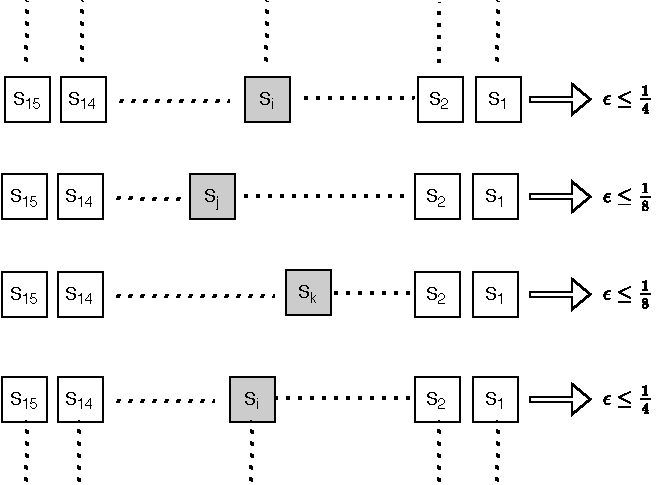
\includegraphics[width=\linewidth]{LC1.pdf}
        \endminipage
        \caption{Bias Calculation}
    \end{figure}
    
\end{frame}

\begin{frame}{Outline of the Proof Cont..}
\begin{itemize}
    \item Bias Calculation : 
    \begin{equation*}
        \epsilon_4^{(4)} \leq 2^{4-1} \times (2^{-2})^2 \times (2^{-3})^2
    \end{equation*}
    \begin{equation*}
        \epsilon_4^{(4)} \leq 2^{-7} 
    \end{equation*}
    \item Case 2 : 5 Active S-boxes involved
    \begin{equation*}
        \epsilon_4^{(5)} \leq 2^{5-1} \times (2^{-2})^4 \times (2^{-3})
    \end{equation*}
    \begin{equation*}
        \epsilon_4^{(5)} \leq 2^{-7} 
    \end{equation*}
    \item Case 3 : More than 5 Active S-boxes involved
    \begin{equation*}
        \epsilon_4^{(i)} \leq 2^{i-1} \times (2^{-2})^i \;\; for \;\; i > 5
    \end{equation*}
    Detailed Proof is given in the report.
\end{itemize}
\end{frame}

\begin{frame}{Requirements for a Successful LC attack}
\begin{itemize}
    \item Maximal Bias of 28-round linear approximation 
    \begin{equation*}
        \epsilon_{28} \leq 2^{6} \times \epsilon_4^{7} = 2^6 \times (2^{-7})^7 \implies \epsilon_{28} \leq 2^{-43}
    \end{equation*}
    \item Assuming the cryptanalyst needs to approximate only 28 Rounds.
    \item Even for single bit key recovery, $N = c|\epsilon|^{-2}$, where constant $c \geq 2$ known plain-texts are required.
    \item Thus, $2^{86}$ known plain-texts are required. 
    \item The data requirement exceeds the total plain-text space available, which is $2^{64}$. 
    \item PRESENT-80 is resistant to Linear attack.
\end{itemize}
    
\end{frame}
\section{Correlation Analysis}
\begin{frame}{The Experiment}
\begin{itemize}
    \item Correlation between the encryption time of PRESENT algorithm and the number of set bits in the key.
    \item Generate random messages of 64 bit and corresponding to each message generate random keys with count of set bits varying from 1 to 79.
\end{itemize}
\end{frame}
\begin{frame}{The Experiment Cont..}
\begin{center}
        \begin{figure}[h!]
            \minipage{0.5\textwidth}
              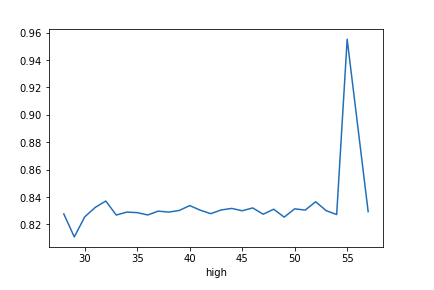
\includegraphics[width=0.8\linewidth]{CA1.PNG}
            \endminipage\hfill
            \minipage{0.5\textwidth}
              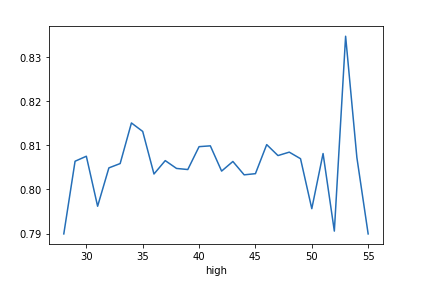
\includegraphics[width=0.8\linewidth]{CA2.PNG}
            \endminipage
        \end{figure}
    \end{center}
    \begin{center}
        \begin{figure}[h!]
            \minipage{0.5\textwidth}
              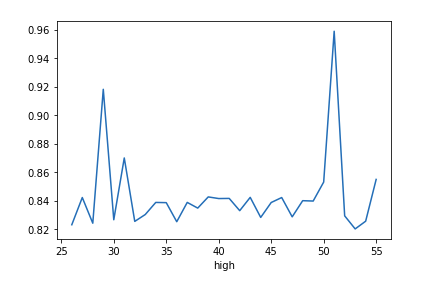
\includegraphics[width=0.8\linewidth]{CA3.PNG}
            \endminipage\hfill
            \minipage{0.5\textwidth}
              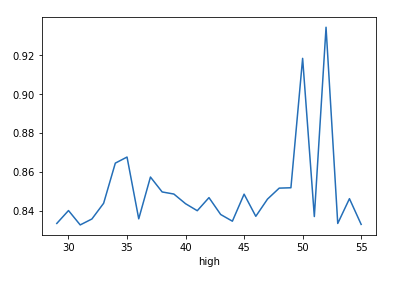
\includegraphics[width=0.8\linewidth]{CA4.PNG}
            \endminipage
        \end{figure}
    \end{center}
\end{frame}
\begin{frame}{The Experiment Cont..}
\begin{center}
        \begin{figure}[h!]
            \minipage{0.5\textwidth}
              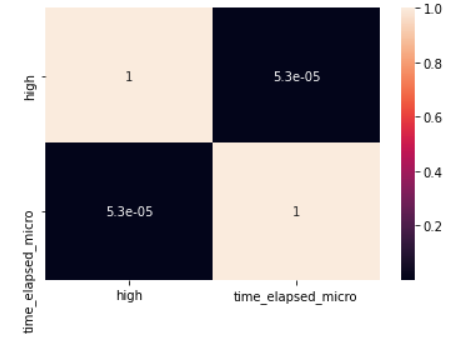
\includegraphics[width=0.8\linewidth]{heatmap.PNG}
            \endminipage\hfill
            \minipage{0.5\textwidth}
              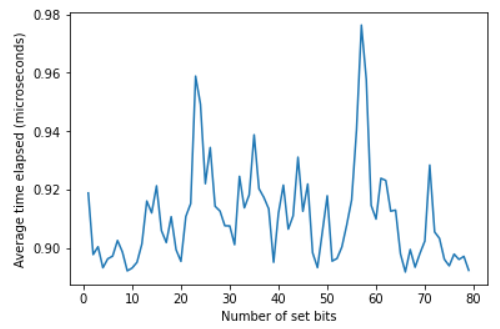
\includegraphics[width=0.8\linewidth]{lineplot.PNG}
            \endminipage
        \end{figure}
    \end{center}
\begin{itemize}
    \item Near to zero correlation exists.
    \item No or very weak linear relationship between the variables.
\end{itemize}
\end{frame}
\section{Brownie Point Nominations}

\begin{frame}{Brownie Points}
\begin{block}{Implementation of DC of Reduced Round PRESENT Cipher}
        We could not find any implementation of Differential analysis on the round reduced version of PRESENT. So, using the idea of differential and filtering taught in the course, we have implemented a differential attack on 3 Rounds of PRESENT. 
\end{block}
\end{frame}
\begin{frame}{Brownie Points Cont..}
    \begin{block}{Correlation Analysis}
        We experimented on various side-channel characteristics of PRESENT that could affect the run time of encryption function. Although on initial experimentation, we found some correlation between number of bits high in the key and the time taken for encryption. But, on randomising the messages also, we could not find any effective correlation. We believe that, this should be further experimented, as there are no paper available on this topic.
\end{block}
\end{frame}
\section{Conclusion}

\begin{frame}{Conclusion}
\begin{itemize}
    \item Understanding the design choices of PRESENT cipher. 
    \item Properties of S-box
    \item Resistance against cryptographic attacks
    \item Analysis of theoretical differential attack on 16-rounds PRESENT
    \item Implementation of 3-Rounds differential attack
    \item Linear Cryptanalysis
    \item Side channel Attack developed by us
\end{itemize}

% We started by examining the design choices made while developing the PRESENT cipher. We looked into the various properties that the S-box of present satisfies and the properties that provide resistance against various cryptographic attack. We examined a differential attack on 16-round version of PRESENT. Implementing this attack was not feasible because of the time complexity and high computation power required. So we implemented our own 3-Round differential attack by using the properties discovered by authors of differential analysis on 16-round PRESENT. We experimented
\end{frame}


\begin{frame}{Thanks}
\begin{block}{Team Members}
	\begin{itemize}
		\item Abhishek Shingane
		\item Gopal Ramesh Dahale
		\item Kumari Rani
	\end{itemize}
\end{block}
\begin{block}{Implementation Info}
	\begin{itemize}
		\item Github Link: \href{https://github.com/Code-Blooded-Human/Present-Cipher}{Present-Cipher}
	\end{itemize}
\end{block}
\end{frame}

\end{document}